\documentclass{article}
\usepackage{graphicx}
\usepackage[margin=2cm]{geometry}
\usepackage{polski}
\input{setup}
\title{Wstęp do spintroniki - tranzystor spinowy.}
\author{Marta Wleklińska}
\date{\today}

\begin{document}

\maketitle

%%%%%%%%%%%%%%%%%%%%%%%%%%%%%%%%%%%%%%%%
\section{Wstęp}
%%%%%%%%%%%%%%%%%%%%%%%%%%%%%%%%%%%%%%%%
%%%%%%%%%%%%%%%%%%%%%%%%%%%%%%%%%%%%%%%%
W ćwiczeniu analizowano nanourządzenia spintroniki.
Ponownie korzystano z pakietu \texttt{Kwant}, którym po zdefiniowaniu układu, mogliśmy badać jego parametry: np. relacje dyspersji w obecnościach różnych pól magnetycznych, konduktancje, transmitancje.

%%%%%%%%%%%%%%%%%%%%%%%%%%%%%%%%%%%%%%%%
%%%%%%%%%%%%%%%%%%%%%%%%%%%%%%%%%%%%%%%%
\section{Wyniki}
%%%%%%%%%%%%%%%%%%%%%%%%%%%%%%%%%%%%%%%%
%%%%%%%%%%%%%%%%%%%%%%%%%%%%%%%%%%%%%%%%
\subsection{Precesja spinu w zewnętrznym polu magnetycznym}
%%%%%%%%%%%%%%%%%%%%%%%%%%%%%%%%%%%%%%%%
W pierwszym ćwiczeniu badaliśmy precesję spinu w zewnętrznym polu magnetycznym.
Rozpatrywany układ był nanodrutem 2D o długości $L$ i szerokości $W$.
Na rysunku~\ref{fig:ex1-rel-dysp-woB} została przedstawiona relacja dyspersji takiego układu.
%%%%%%%%%%%%%%%%%%%%%%%%%%%%%%%%%%%%%%%%
\begin{figure}[htp!]
    \centering
    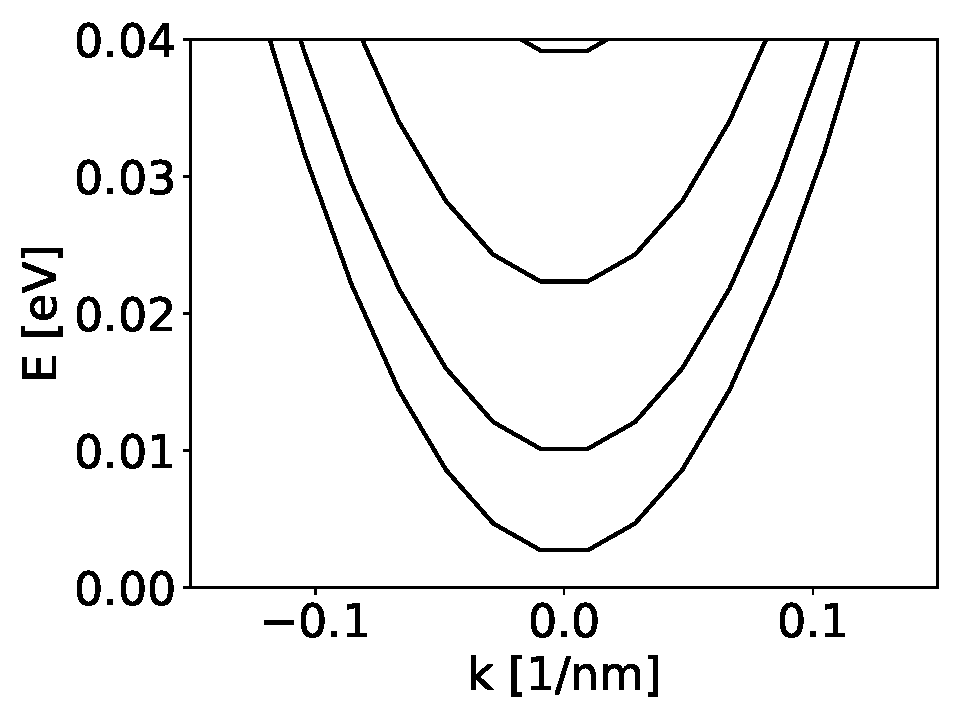
\includegraphics[width=0.65\linewidth]{ex1/disp_wo_B_ex1.pdf}
    \caption{Relacja dyspersji $E(k)$ dla $B = 0$}
    \label{fig:ex1-rel-dysp-woB}
\end{figure}
%%%%%%%%%%%%%%%%%%%%%%%%%%%%%%%%%%%%%%%%
W~kolejnym kroku wprowadziliśmy pole magnetyczne - skierowane dla kolejnych kierunków $x, y, z$.
Na rysunku~\ref{fig:ex1-relacja-dyspersji} zostały zapisane ponownie relacje dyspersji przy przyłożonym polu.
\begin{figure}[htp!]
    \centering
\begin{subfigure}{.32\textwidth}
    \centering
    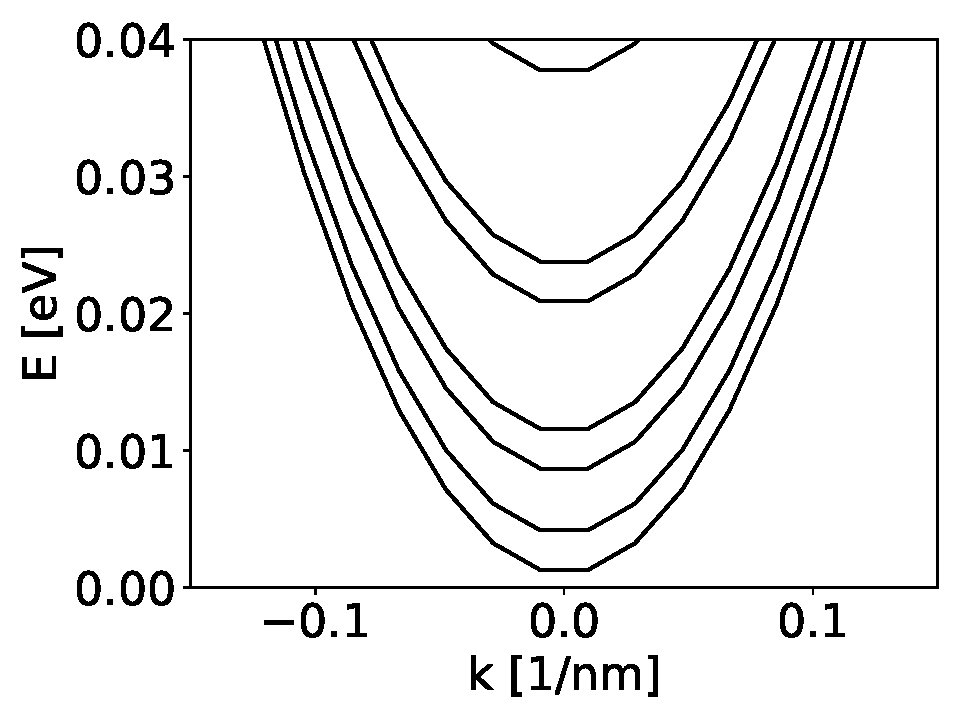
\includegraphics[width = 1.0\textwidth]{ex1/disp_ex1_Bx1.pdf}
    \caption{}
    \label{fig:disp_ex1_Bx1}
\end{subfigure}
\begin{subfigure}{.32\textwidth}
    \centering
    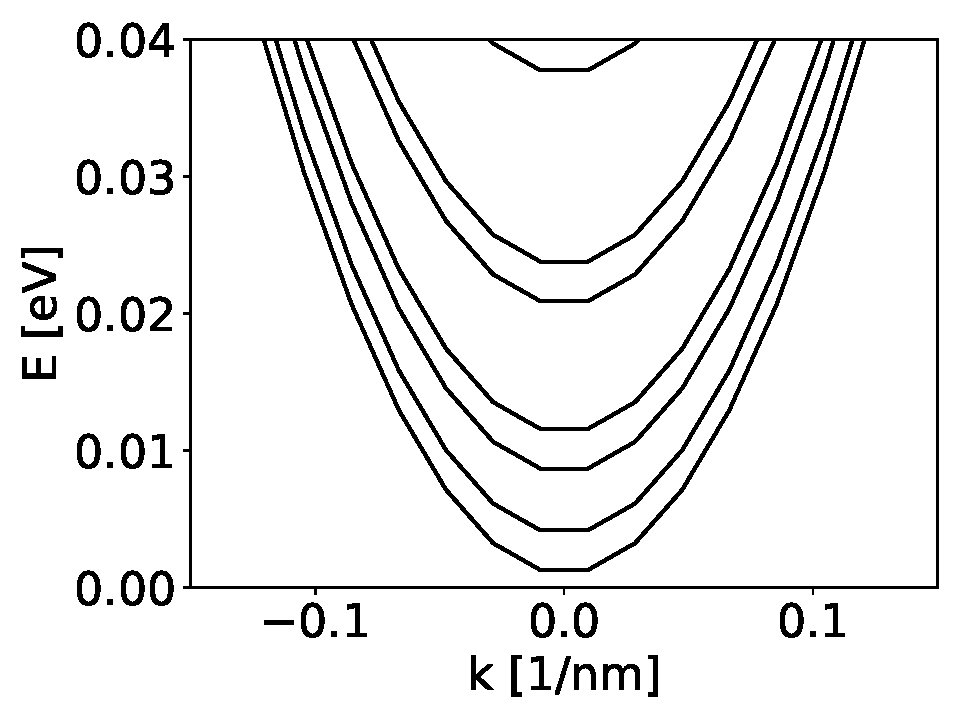
\includegraphics[width = 1.0\textwidth]{ex1/disp_ex1_Bx2.pdf}
    \caption{}
    \label{fig:disp_ex1_Bx2}
\end{subfigure}
\begin{subfigure}{.32\textwidth}
    \centering
    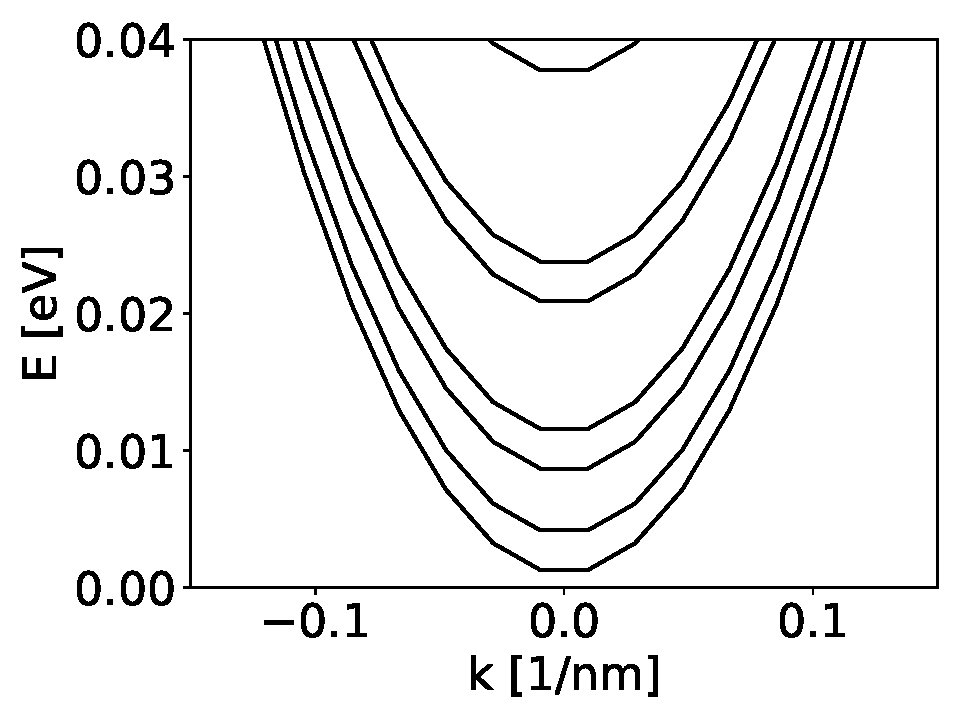
\includegraphics[width = 1.0\textwidth]{ex1/disp_ex1_Bz.pdf}
    \caption{}
    \label{fig:disp_ex1_Bz}
\end{subfigure}
\caption{Relacje dyspersji $E(k)$ dla (\textbf{(a)})~$\mathbf{B} = (B \ 0 \ 0)$, (\textbf{(b)})~$\mathbf{B} = (0 \ B \ 0)$, (\textbf{(c)})~$\mathbf{B} = (0 \ 0 \ B)$, przy $b = 1$~T}
\label{fig:ex1-relacja-dyspersji}
\end{figure}
%%%%%%%%%%%%%%%%%%%%%%%%%%%%%%%%%%%%%%%%
W porównaniu do rysunku~\ref{fig:ex1-rel-dysp-woB} obserwujemy dla każdego z rysunków~\ref{fig:disp_ex1_Bx1},~\ref{fig:disp_ex1_Bx2},~\ref{fig:disp_ex1_Bz} więcej modów.
Obserwujemy rozszczepienie Zeemana, które nie zależy od kierunku przyłożenia pola (dla każdego $x, y, z$) relacja dyspersji ma ten sam kształt.\\
\\
Następnie ustaliliśmy pole $\mathbf{B} = (0 \ 0 \ B_z)$ i wyznaczyliśmy zależność konduktancji w funkcji energii na rysunku~\ref{fig:conductance_ex1}.
Przez pojawianie się kolejnych modów przez rozszczepienie Zeemana (rys.~\ref{fig:disp_ex1_Bz}) schodki konduktancji $2e^2/h$.\\
%%%%%%%%%%%%%%%%%%%%%%%%%%%%%%%%%%%%%%%%
\begin{figure}[htp!]
    \centering
    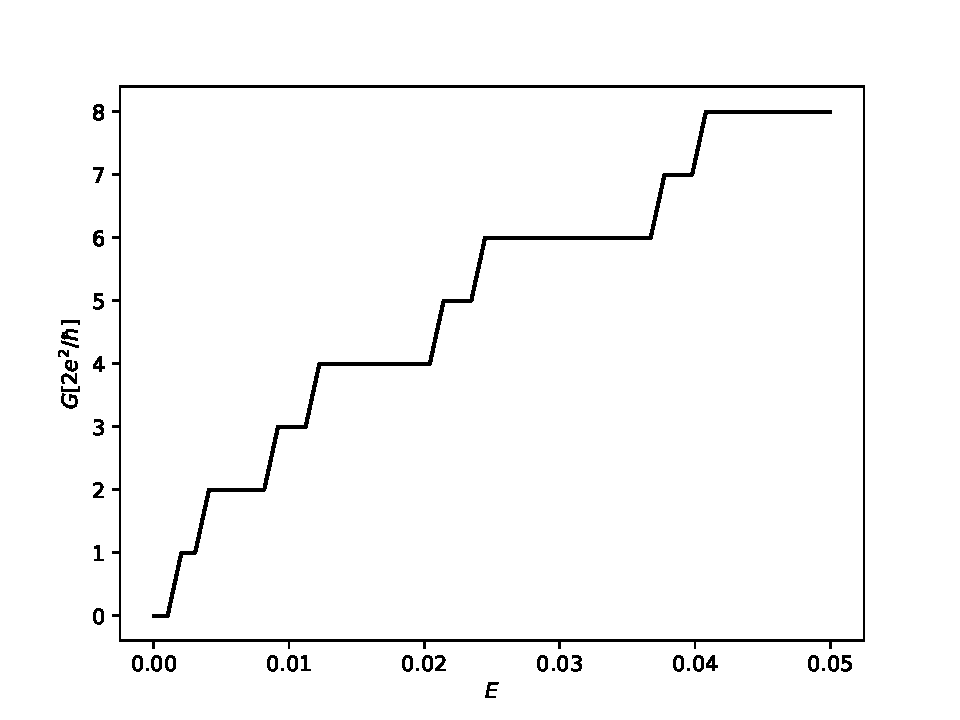
\includegraphics[width=0.65\linewidth]{ex1/ex1_conductance.pdf}
    \caption{Konduktancja w funkcji energii padającego elektronu dla $B_z = 1$~T}
    \label{fig:conductance_ex1}
\end{figure}
%%%%%%%%%%%%%%%%%%%%%%%%%%%%%%%%%%%%%%%%
\\
W kolejnej modyfikacji układu wprowadziliśmy pole $\mathbf{B} = (0 \ B_y \ B_z)$.
Wartość $B_z=0.1$~T jest ustalona podczas gdy wartość $B_y$ przykładaliśmy dla kolejnych wartości $B_y\in[0,1]~$T.
Dodatkowo było ono przyłożone w obszarze $[0.2, 0.8]~L$.
Wyznaczyliśmy zatem wartość współczynników transmitancji dla różnych kombinacji przejść (\texttt{up--down}, \texttt{up--up}, \texttt{down--up}, \texttt{down--down}).
Współczynniki transmisji w funkcji $B_y$ zostały przedstawione na rysunku~\ref{fig:ex1_trans_spin}.
%%%%%%%%%%%%%%%%%%%%%%%%%%%%%%%%%%%%%%%%
\begin{figure}[htp!]
    \centering
    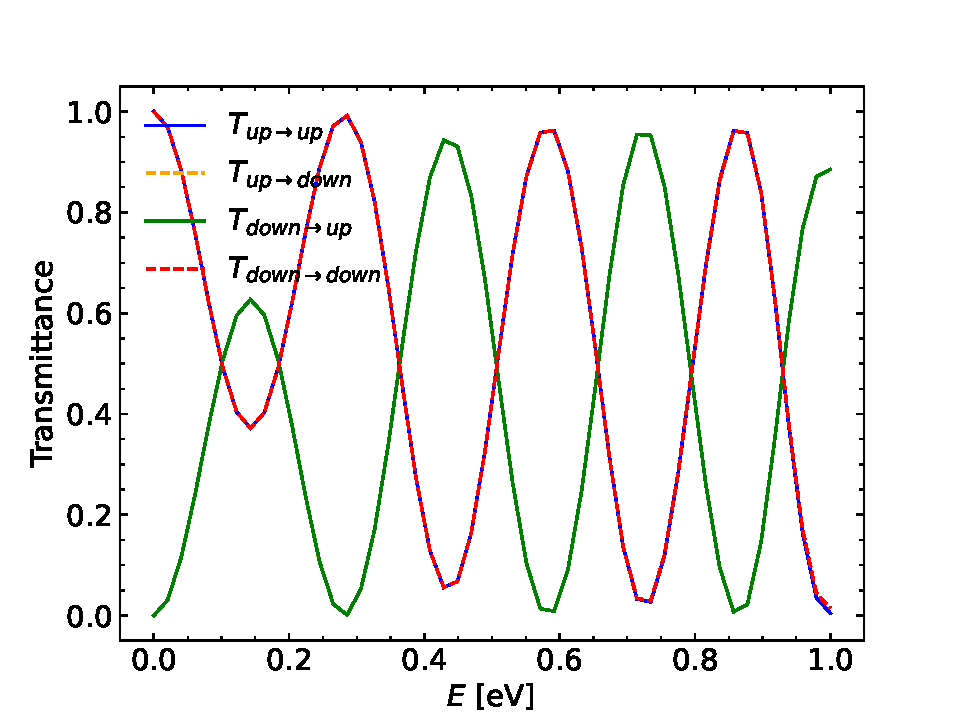
\includegraphics[width=0.65\linewidth]{ex1/ex1_transmittances.pdf}
    \caption{Zależne od spinu współczynniki transmisji w funkcji pola magnetycznego $B_y$ przy $B_z = 1$~T oraz $E = 5$~meV}
    \label{fig:ex1_trans_spin}
\end{figure}
%%%%%%%%%%%%%%%%%%%%%%%%%%%%%%%%%%%%%%%%
Przez precesję spinu zauważamy naprzemiennie minima i maksima współczynników transmisji.
Dla takiego układu ustaliliśmy dodatkowo $B_y=0.6$~T oraz zbadaliśmy gęstość ładunku o spinie \texttt{up, down}, co zostało przedstawione na rysunku~\ref{fig:ex1-spin-density}.
%%%%%%%%%%%%%%%%%%%%%%%%%%%%%%%%%%%%%%%%
\begin{figure}[htp!]
    \centering
\begin{subfigure}{.32\textwidth}
    \centering
    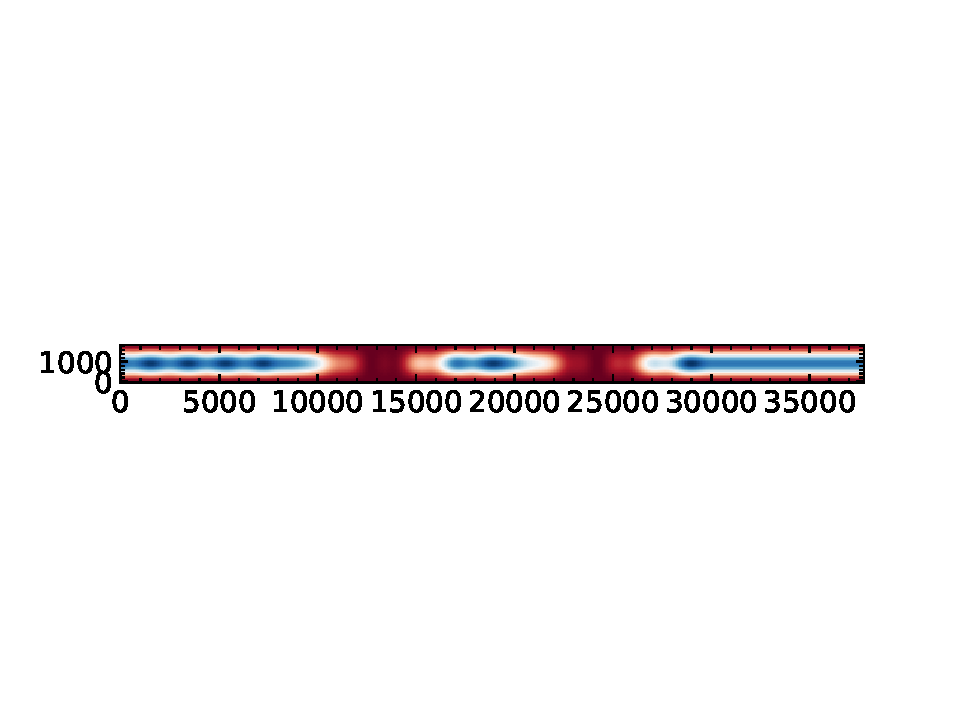
\includegraphics[width = 1.0\textwidth]{ex1/ex1_density_up.pdf}
    \caption{}
    \label{fig:ex1-spin-up}
\end{subfigure}
\begin{subfigure}{.32\textwidth}
    \centering
    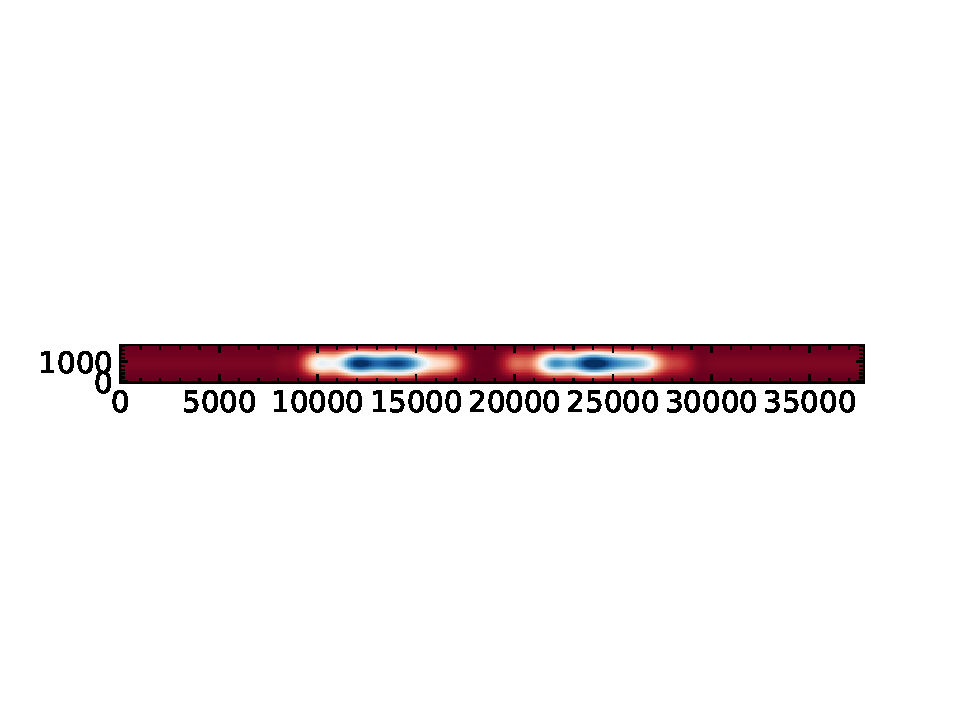
\includegraphics[width = 1.0\textwidth]{ex1/ex1_density_down.pdf}
    \caption{}
    \label{fig:ex1-spin-down}
\end{subfigure}
\caption{Rozkład gęstości elektronów o spinie \textbf{(a)}~\texttt{up} i \textbf{(b)}~\texttt{down} }
\label{fig:ex1-spin-density}
\end{figure}
Ponownie obserwujemy precesję.
Następnie badamy gęstość spinu $s_x, s_y, s_z$, co zostało zapisane na rysunku~\ref{fig:ex1-spin-density-s}.
%%%%%%%%%%%%%%%%%%%%%%%%%%%%%%%%%%%%%%%%
\begin{figure}[htp!]
    \centering
\begin{subfigure}{.495\textwidth}
    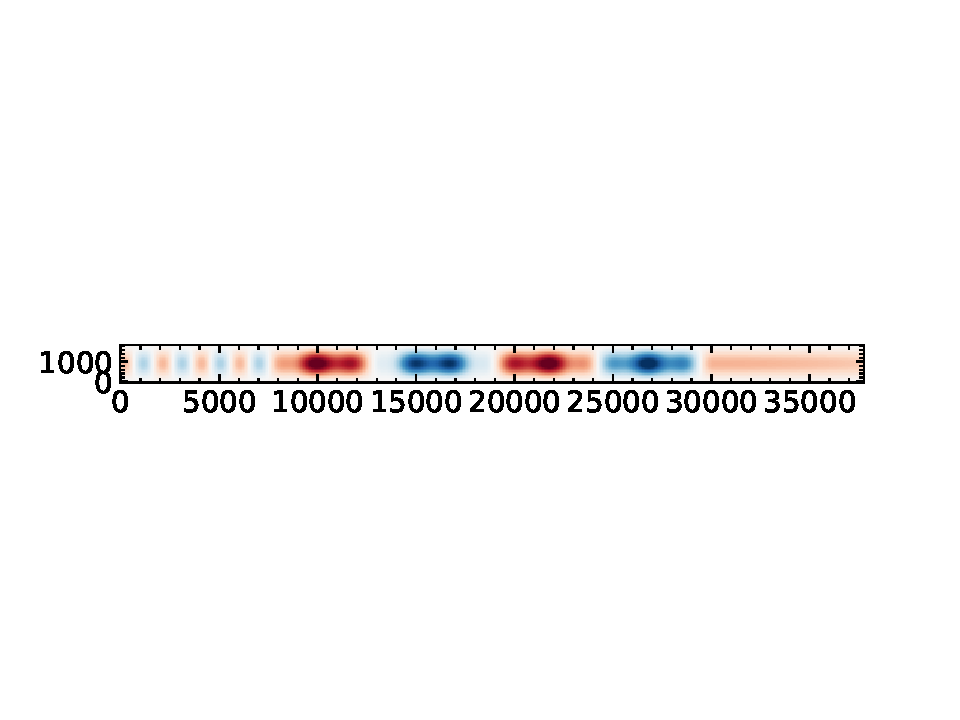
\includegraphics[width=1.0\linewidth]{ex1/ex1_density_x.pdf}
    \caption{}
    \label{fig?:ex1-sx}
\end{subfigure}
\begin{subfigure}{.495\textwidth}
    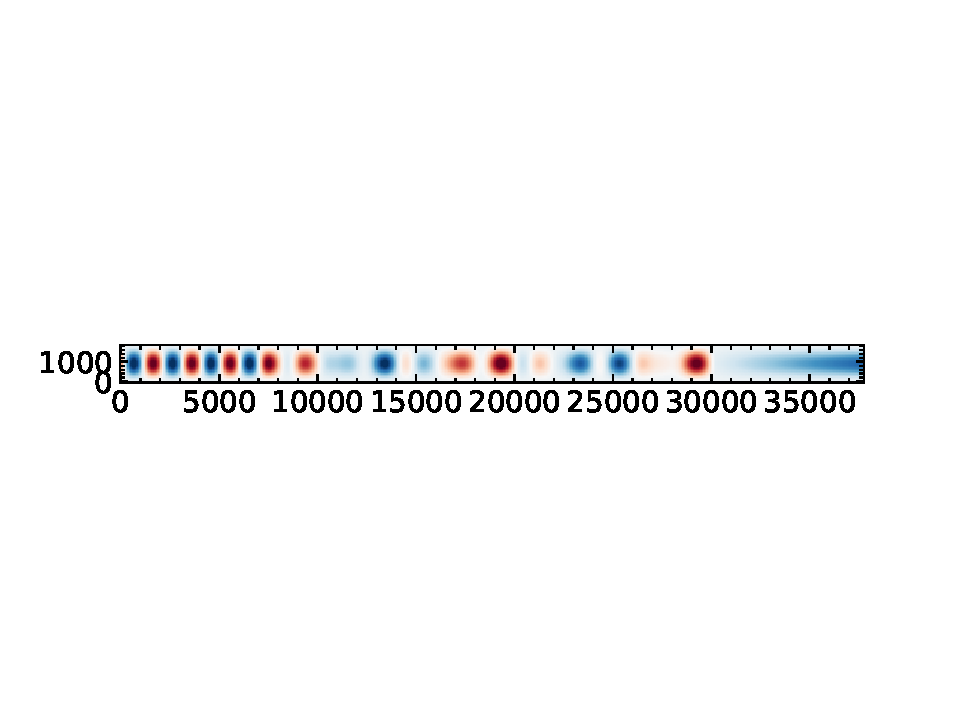
\includegraphics[width=1.0\linewidth]{ex1/ex1_density_y.pdf}
    \caption{}
    \label{fig:ex1-sy}
\end{subfigure}
\begin{subfigure}{.495\textwidth}
    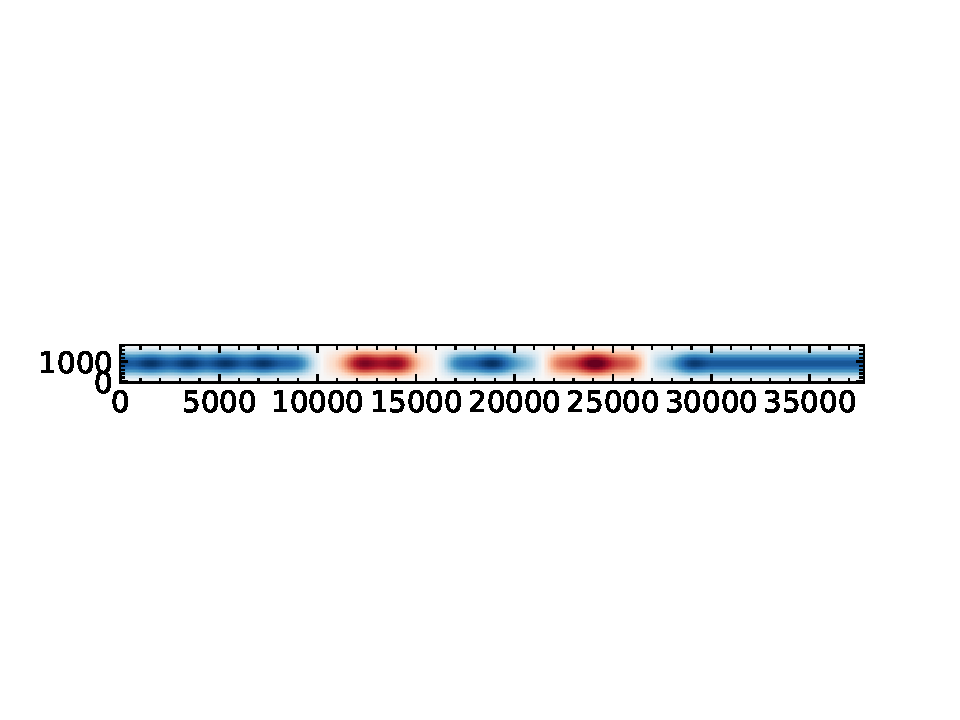
\includegraphics[width=1.0\linewidth]{ex1/ex1_density_z.pdf}
    \caption{}
    \label{fig:ex1-sz}
\end{subfigure}
\caption{Rozkład gęstości spinów $s_x, s_y, s_z$ w nanodrucie przy $B_y = 0.6$~T, $B_z = 0.1$~T, $E = 5$~meV}
\label{fig:ex1-spin-density-s}
\end{figure}
%%%%%%%%%%%%%%%%%%%%%%%%%%%%%%%%%%%%%%%%
Gęstości spinów i gęstości elektronów o odpowiednich spinach to nie to samo, co potwierdzają wyniki.
%%%%%%%%%%%%%%%%%%%%%%%%%%%%%%%%%%%%%%%%
%%%%%%%%%%%%%%%%%%%%%%%%%%%%%%%%%%%%%%%%
\subsection{Tranzystor spinowy oparty na ferromagnetycznych paskach}
%%%%%%%%%%%%%%%%%%%%%%%%%%%%%%%%%%%%%%%%
W kolejnym układzie badaliśmy wpływ pola zewnętrznego $\mathbf{B}_{\text{ext}}$ oraz helikalnego $\mathbf{B}_h = B_h\left[\sin\left(\frac{2\pi(x-x_0)}{a}\right) \ 0 \ \cos\left(\frac{2\pi (x-x_0)}{a}\right)\right]$.
W pierwszym przypadku wyzerowaliśmy wartości $\mathbf{B}_{\text{ext}} = (0 \ 0 \ B_{\text{ext}}=0)$.
Ponownie - wyznaczyliśmy dla takiego układu relację dyspersji, co zostało zapisane na rysunku~\ref{fig:ex3-relacja dyspersji}.
%%%%%%%%%%%%%%%%%%%%%%%%%%%%%%%%%%%%%%%%
\begin{figure}[htp!]
    \centering
\begin{subfigure}{.495\textwidth}
    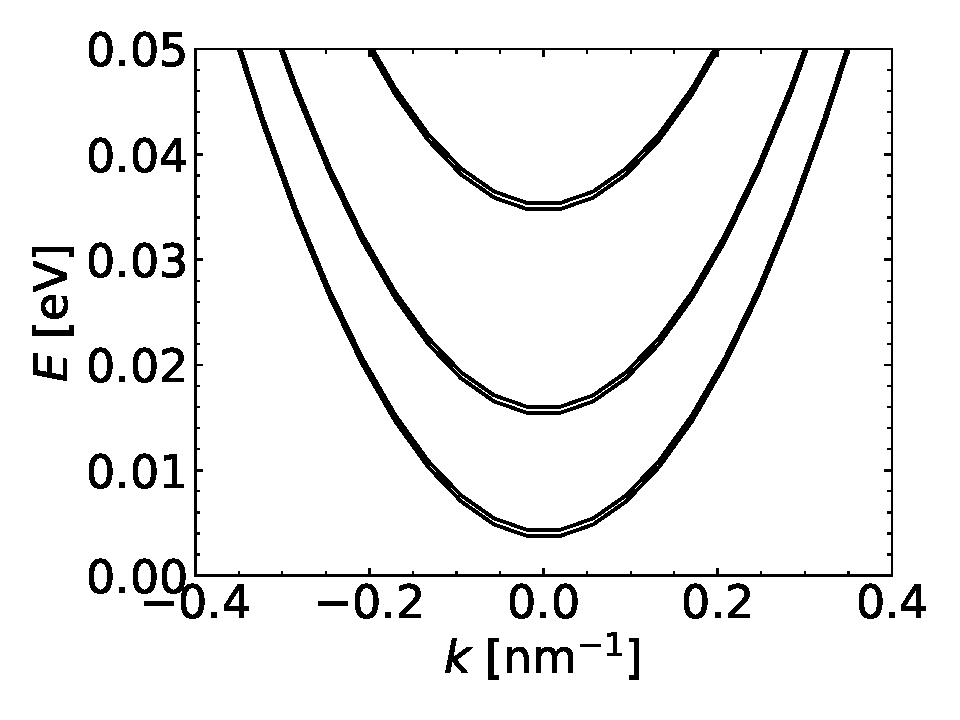
\includegraphics[width=1.0\linewidth]{ex3/ex3_disp_04.pdf}
    \caption{}
    \label{fig:ex3-rel-disp}
\end{subfigure}
\begin{subfigure}{.495\textwidth}
    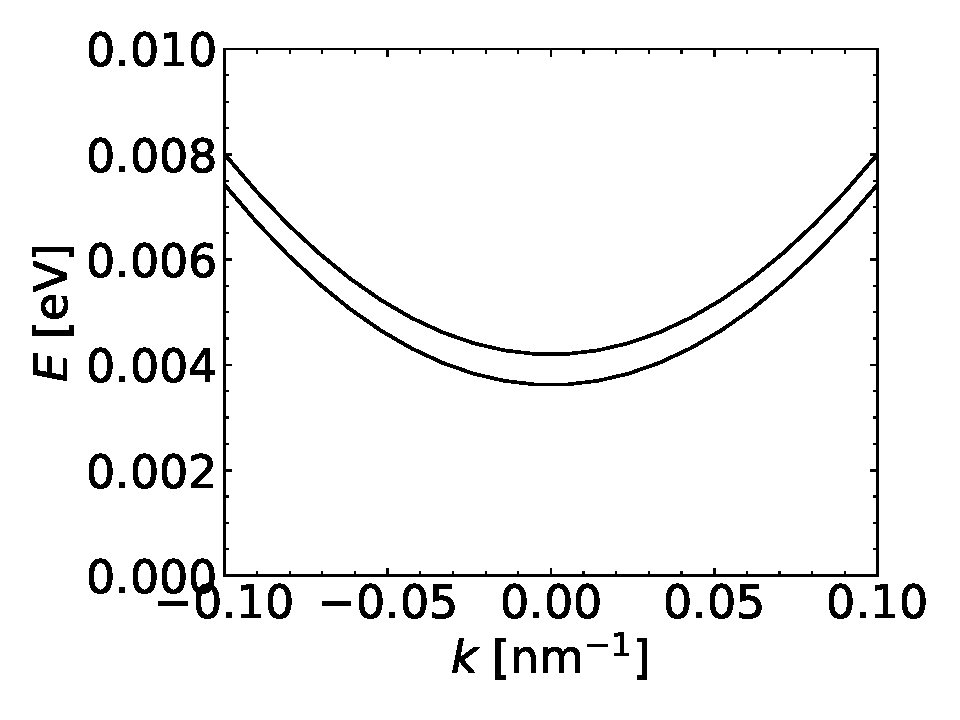
\includegraphics[width=1.0\linewidth]{ex3/ex3_disp.pdf}
    \caption{}
    \label{fig:ex3-rel-disp-przyb}
\end{subfigure}
\caption{Relacja dyspersji $E(k)$ przy $B_{\text{ext}}=0$}
    \label{fig:ex3-relacja dyspersji}
\end{figure}
%%%%%%%%%%%%%%%%%%%%%%%%%%%%%%%%%%%%%%%%
Zauważamy rozszczepienie Zeemana, które widać szczególnie przy przybliżeniu na rysunku~\ref{fig:ex3-rel-disp-przyb}.
W kolejnej modyfikacji, badaliśmy wpływ pola $B_{\text{ext}}$ zmieniając go przy $B_{\text{ext}}\in[0,0.1]$~T.
Przyjęliśmy wartość energii jako połowę spinowo rozszczepionego stanu podstawowego i zapisywaliśmy konduktancję dla danej wartości.
Zależność konduktancji od wartości pola $B_{\text{ext}}$ została przedstawiona na rysunku~\ref{fig:ex3-conductance}.
\begin{figure}[htp!]
    \centering
    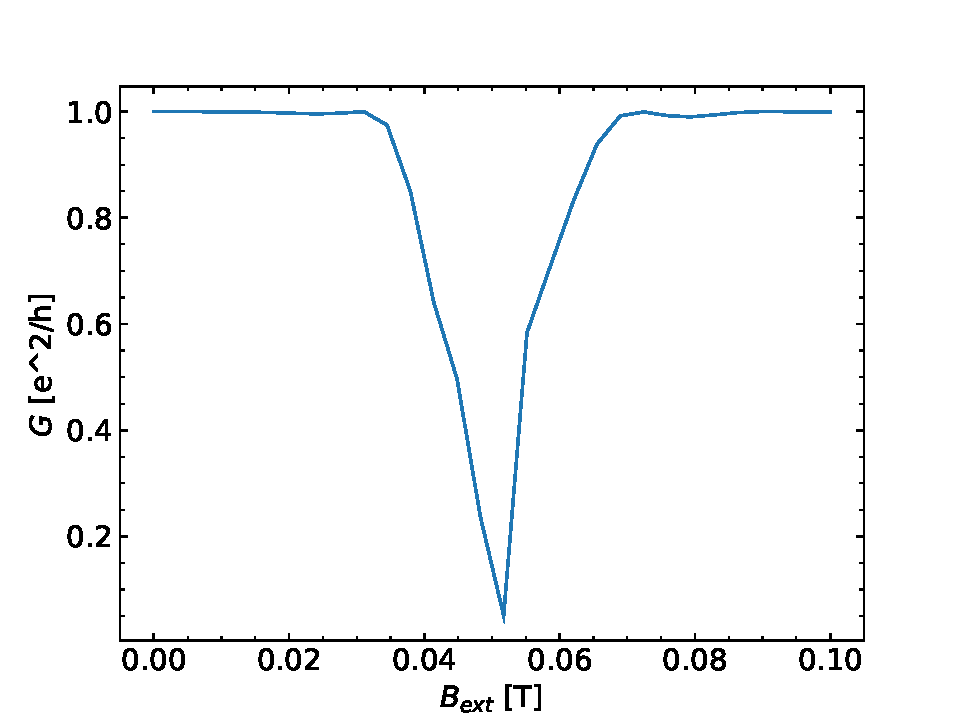
\includegraphics[width=0.5\linewidth]{ex3/ex3_conductance_0.pdf}
    \caption{Wykres konduktancji w funkcji zewnętrznego pola magnetycznego $B_{\text{ext}}$ przy $E = 0.004$~eV}
    \label{fig:ex3-conductance}
\end{figure}
%%%%%%%%%%%%%%%%%%%%%%%%%%%%%%%%%%%%%%%%
Zauważamy wartość konduktancji na poziomie 1 przy małych i dużych wartościach $B_{\text{ext}}$.
Obserwujemy jednak nagły spadek konduktancji przy $B_{\text{ext}}\sim 0.05$~mT, które jest równe wartości $B_h$.
%%%%%%%%%%%%%%%%%%%%%%%%%%%%%%%%%%%%%%%%
\subsection{Tranzystor spinowy oparty na oddziaływaniu spin-orbita}
%%%%%%%%%%%%%%%%%%%%%%%%%%%%%%%%%%%%%%%%
Ostatni układ jaki został analizowany był tranzystor spinowy oparty na oddziaływaniu spin--orbita.
Zatem zamiast przykładania pola magnetycznego w tranzystorach (co by zwiększyło jego rozmiar), chcieliśmy sterować spinem poprzez oddziaływanie spin-orbita typu Rashby.
Parametrem opisującym własności transportowe będzie $\alpha$.
W pierwszej kolejności wyznaczyliśmy relację dyspersji, co zostało przedstawione na rysunku~\ref{fig:ex2-so-disp}.
%%%%%%%%%%%%%%%%%%%%%%%%%%%%%%%%%%%%%%%%
\begin{figure}[htp!]
    \centering
    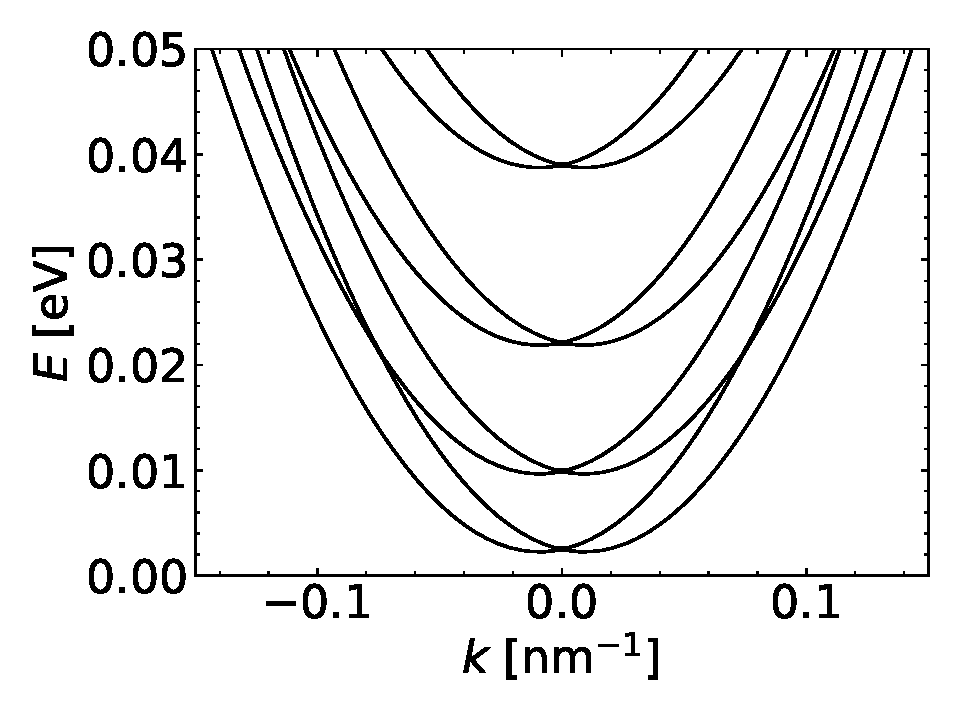
\includegraphics[width=0.65\linewidth]{ex2/ex2_disp.pdf}
    \caption{Relacje dyspersji $E(k)$ w kanale z uwzględnieniem oddziaływania spin--orbita}
    \label{fig:ex2-so-disp}
\end{figure}
%%%%%%%%%%%%%%%%%%%%%%%%%%%%%%%%%%%%%%%%
Obserwujemy przesunięte paraboliczne relacje w kierunku dodatnich i ujemnych $k$.
Następnie badaliśmy konduktancję w funkcji padającego elektronu - rys.~\ref{fig:ex2-conduct}.
%%%%%%%%%%%%%%%%%%%%%%%%%%%%%%%%%%%%%%%%
\begin{figure}[htp!]
    \centering
    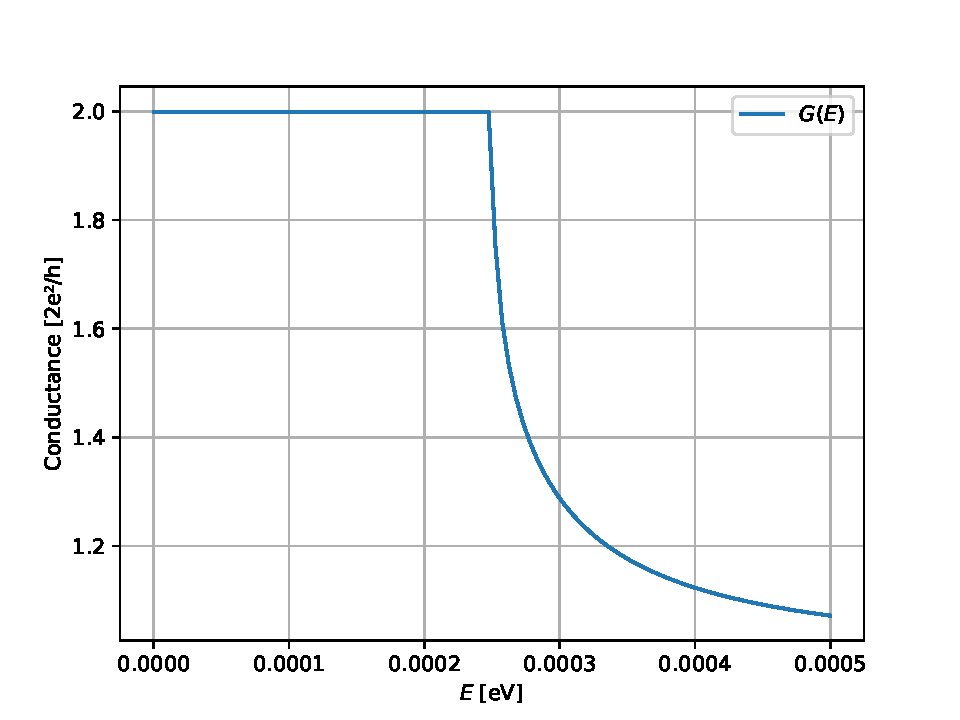
\includegraphics[width=0.65\linewidth]{ex2/ex2_conductance.pdf}
    \caption{Konduktancja w funkcji energii padającego elektronu}
    \label{fig:ex2-conduct}
\end{figure}
%%%%%%%%%%%%%%%%%%%%%%%%%%%%%%%%%%%%%%%%
Zauważamy kolejne schodki konduktancji.\\
\\
W kolejnej części wyznaczyliśmy współczynniki transmisji dla różnych kombinacji przejść elektronu w funkcji parametru $\alpha$.
Przyjęliśmy oddziaływanie spin--orbita w obszarze $0.2, 0.8$~L.
Wyniki zostały zapisane na rysunku~\ref{fig:ex2-trans}.
%%%%%%%%%%%%%%%%%%%%%%%%%%%%%%%%%%%%%%%%
\begin{figure}[htp!]
    \centering
    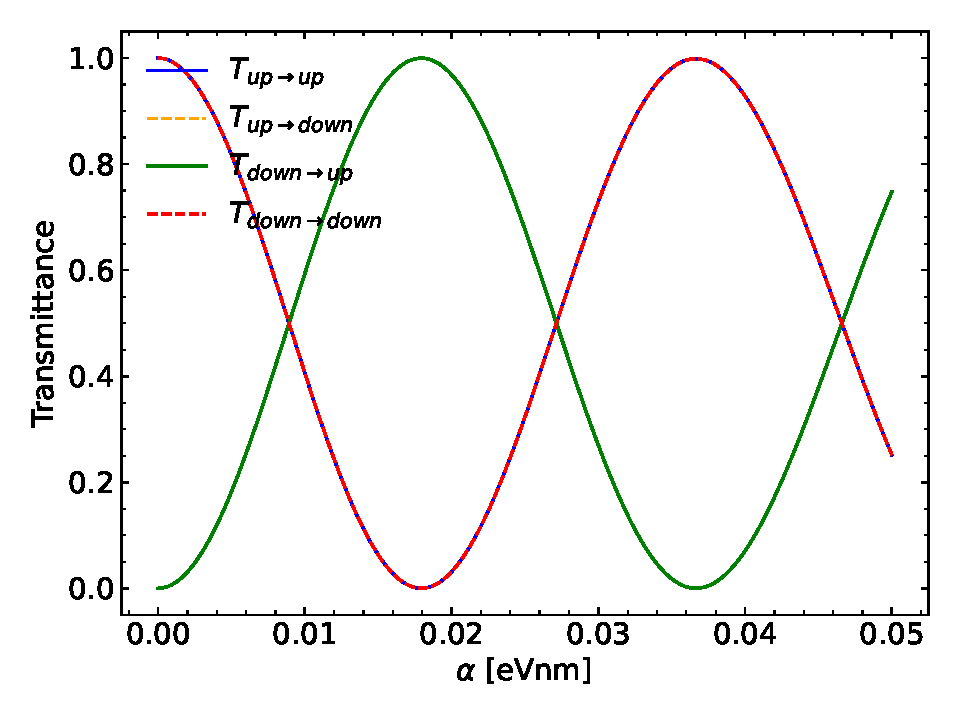
\includegraphics[width=0.65\linewidth]{ex2/ex2_transmittances.pdf}
    \caption{Zależne od spinu współczynniki transmisji w funkcji parametru $\alpha$ przy $E = 5$~meV}
    \label{fig:ex2-trans}
\end{figure}
%%%%%%%%%%%%%%%%%%%%%%%%%%%%%%%%%%%%%%%%
Ponownie występują oscylacyjny charakter krzywych.
Wyraźnie widać, że dla niektórych wartości $\alpha$ elektron zmienia spin na przeciwny.\\
\\
Analizowaliśmy konduktancje $G, G^{\text{up}}, G^{\text{down}}$ dla różnych wartościach polaryzacji kontaktów $P=\{0.2, 0.4, 1.\}$.
Wyniki zostały zapisane na rysunku~\ref{fig:ex2-conduct-p}.
%%%%%%%%%%%%%%%%%%%%%%%%%%%%%%%%%%%%%%%%
\begin{figure}[htp!]
    \centering
\begin{subfigure}{.32\textwidth}
    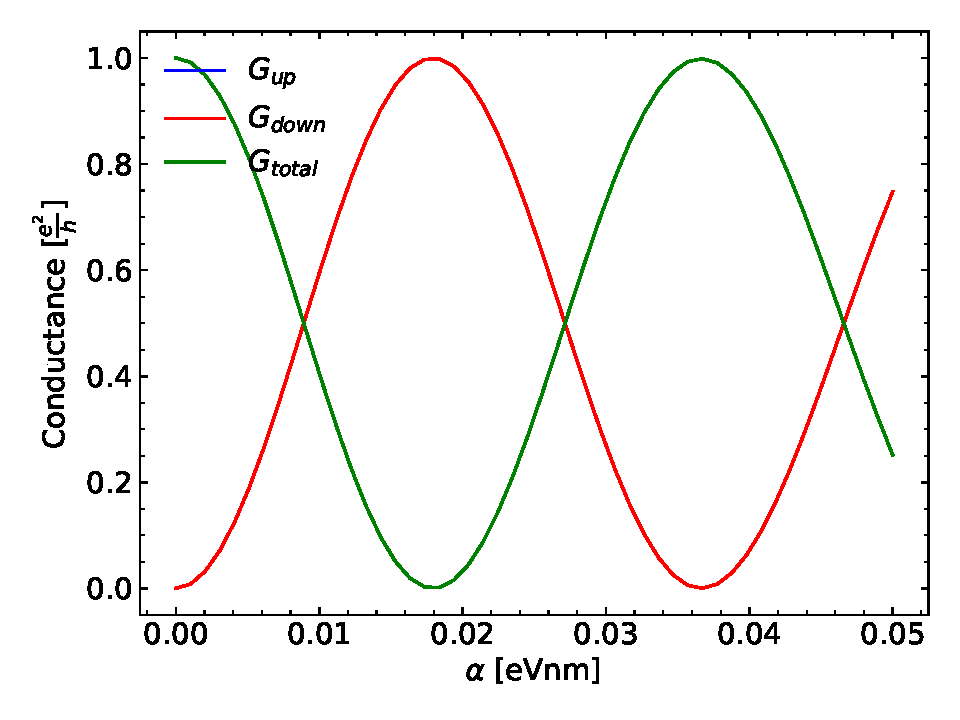
\includegraphics[width = 1.0\textwidth]{ex2/ex_2_cond_p=1.pdf}
    \caption{}
\end{subfigure}
\begin{subfigure}{.32\textwidth}
    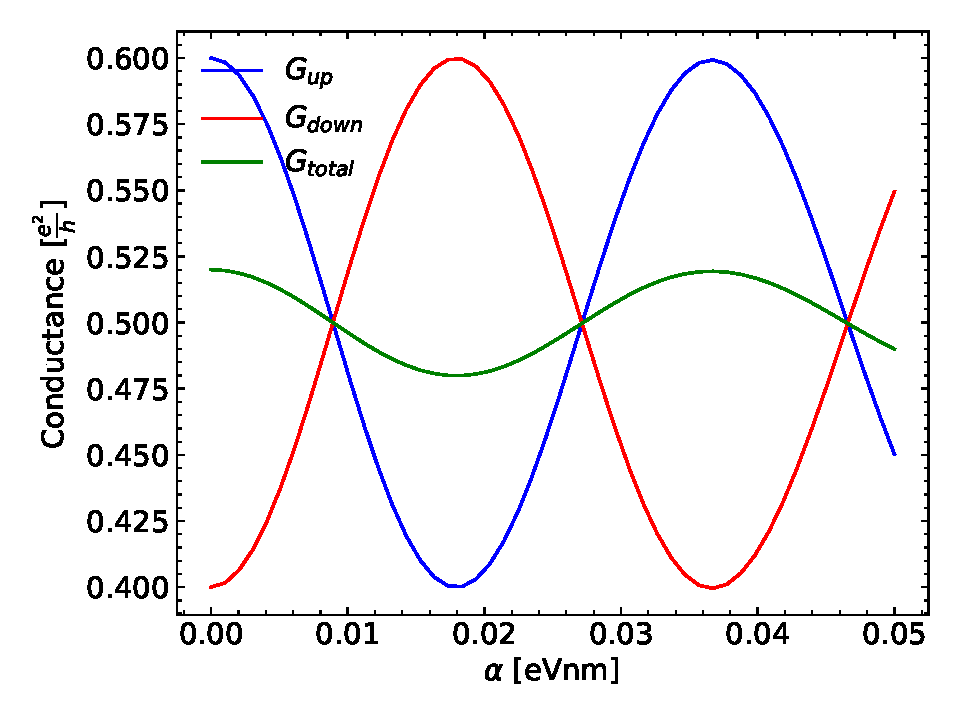
\includegraphics[width = 1.0\textwidth]{ex2/ex_2_cond_p=0.2.pdf}
    \caption{}
\end{subfigure}
\begin{subfigure}{.32\textwidth}
    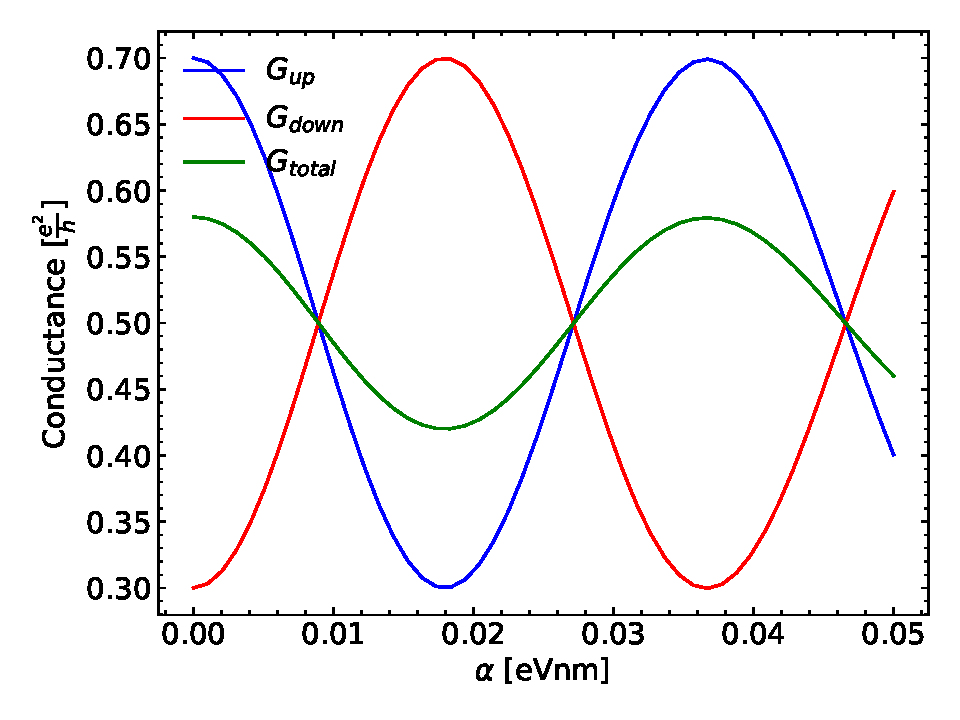
\includegraphics[width = 1.0\textwidth]{ex2/ex_2_cond_p=0.4.pdf}
    \caption{}
\end{subfigure}
    \caption{Zależna od spinu konduktancja oraz konduktancja całkowita funkcji parametru $\alpha$ przy $E = 5$~meV dla \textbf{(a)}~$P=1$; \textbf{(b)}~$P = 0.2$, \textbf{(c)}~$P = 0.4$}
    \label{fig:ex2-conduct-p}
\end{figure}
%%%%%%%%%%%%%%%%%%%%%%%%%%%%%%%%%%%%%%%%
Dla wartości $\alpha$ odpowiadającej całkowitemu obrotowi spinu, zapisaliśmy gęstość elektronu~\ref{fig:spin-density-ex2} oraz gęstość spinu~\ref{fig:ex3-spin-density-s}.
%%%%%%%%%%%%%%%%%%%%%%%%%%%%%%%%%%%%%%%%
\begin{figure}[htp!]
    \centering
\begin{subfigure}{.495\textwidth}
    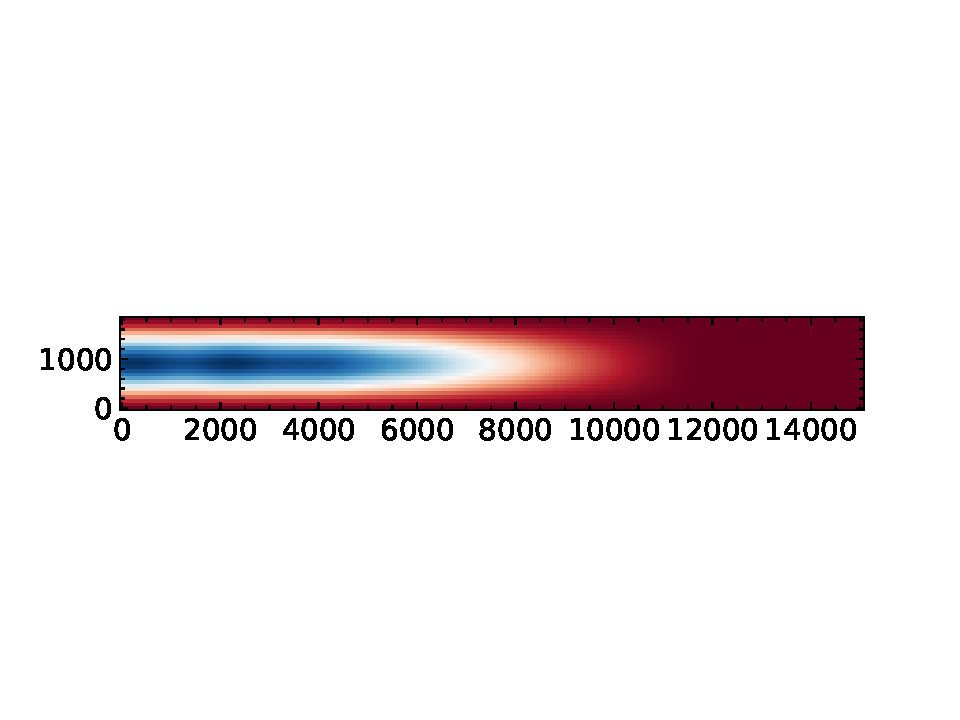
\includegraphics[width=1.0\linewidth]{ex2/ex2_density_up.pdf}
    \caption{}
    \label{fig:ex2-spin-up}
\end{subfigure}
\begin{subfigure}{.495\textwidth}
    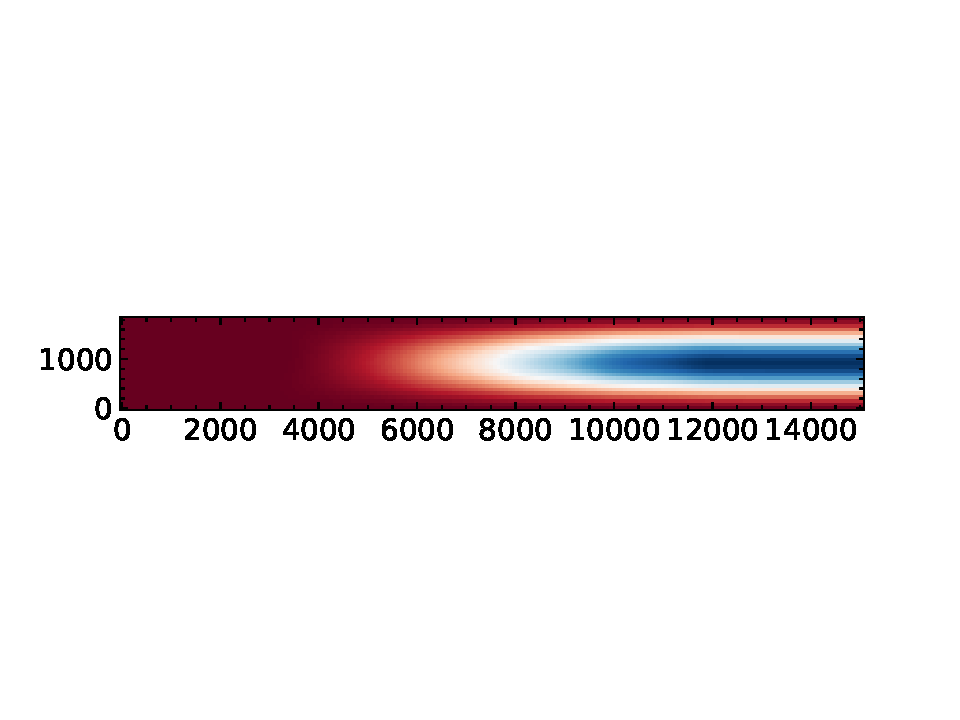
\includegraphics[width=1.0\linewidth]{ex2/ex2_density_down.pdf}
    \caption{}
    \label{fig:ex2-spin-down}
\end{subfigure}
\caption{Zależna od spinu gęstość ładunku w nanourządzeniu przy $E = 5$~meV \textbf{(a)}~spin up \textbf{(b)}~spin down}
\label{fig:spin-density-ex2}
\end{figure}
%%%%%%%%%%%%%%%%%%%%%%%%%%%%%%%%%%%%%%%%
\begin{figure}[htp!]
    \centering
\begin{subfigure}{.32\textwidth}
    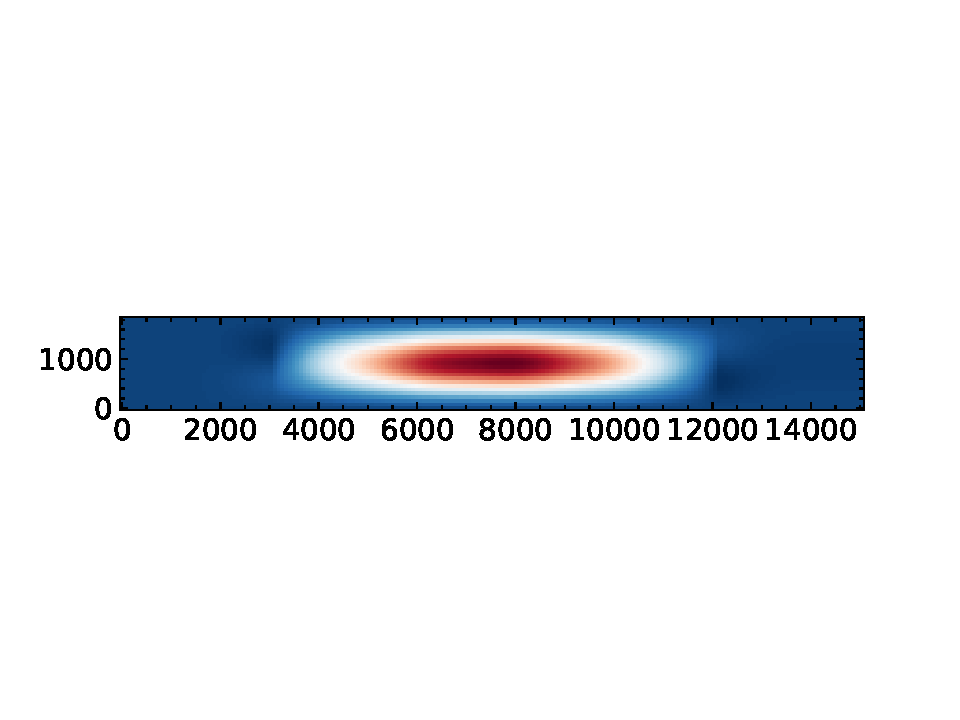
\includegraphics[width=1.0\linewidth]{ex2/ex2_density_x.pdf}
    \caption{}
    \label{fig:ex2-spin-sx}
\end{subfigure}
\begin{subfigure}{.32\textwidth}
    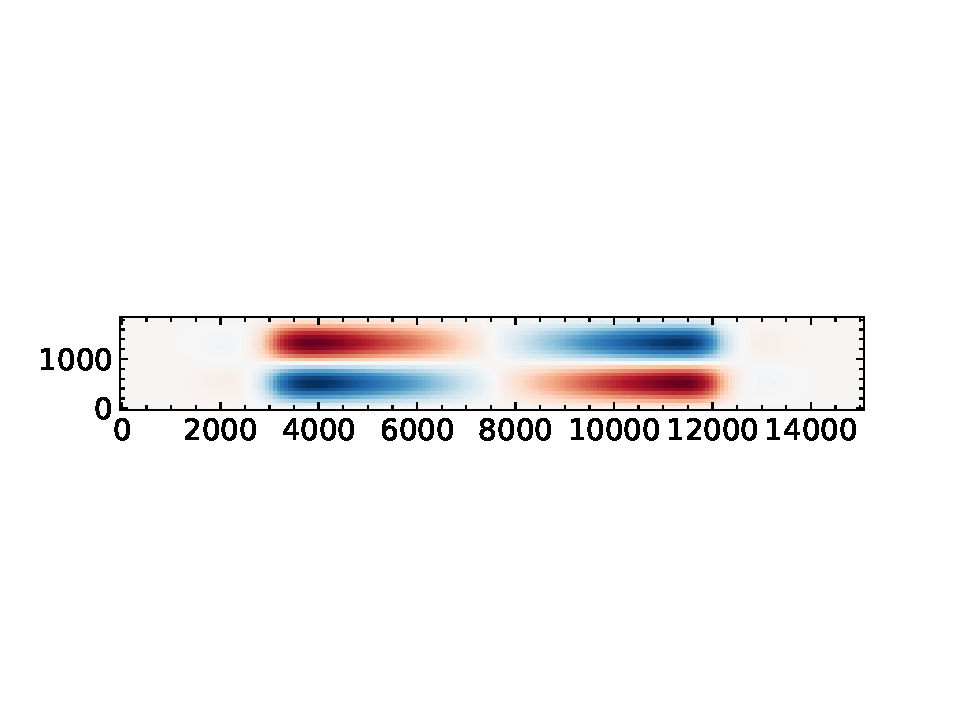
\includegraphics[width=1.0\linewidth]{ex2/ex2_density_y.pdf}
    \caption{}
    \label{fig:ex2-spin-sy}
\end{subfigure}
\begin{subfigure}{.32\textwidth}
    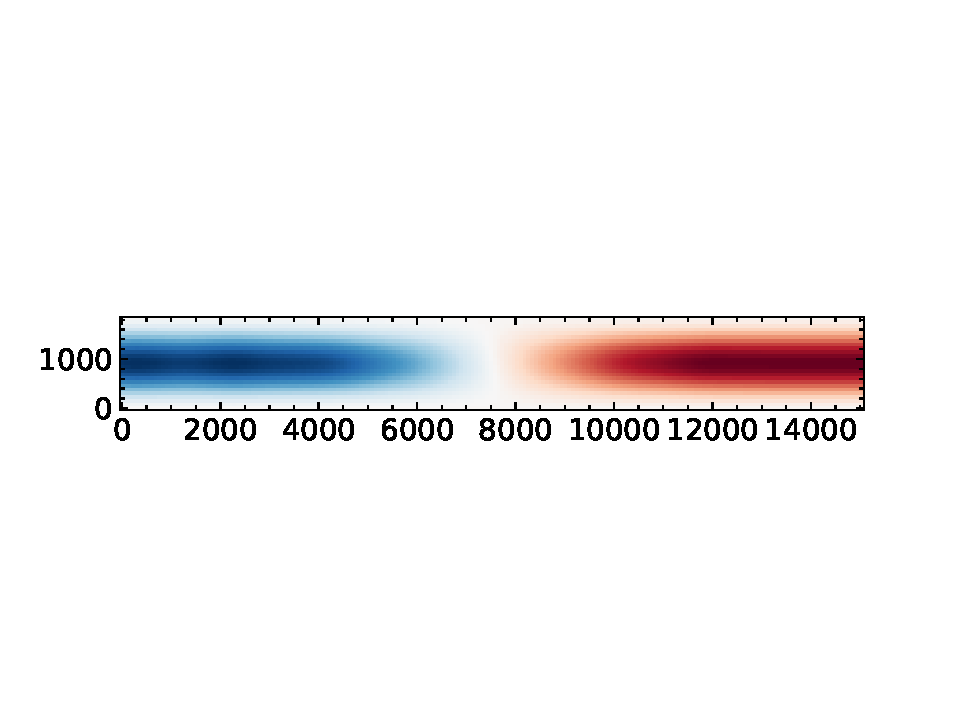
\includegraphics[width=1.0\linewidth]{ex2/ex2_density_z.pdf}
    \caption{}
    \label{fig:ex2-spin-sz}
\end{subfigure}
\caption{Gęstość spinu w nanourządzeniu przy $E = 5$~meV \textbf{(a)}~$s_x$, \textbf{(b)}~$s_y$, \textbf{(c)}~$s_z$}
\label{fig:ex3-spin-density-s}
\end{figure}
Wyraźnie zauważamy zmianę spinu w środku układu.
%%%%%%%%%%%%%%%%%%%%%%%%%%%%%%%%%%%%%%%%
\newpage
%%%%%%%%%%%%%%%%%%%%%%%%%%%%%%%%%%%%%%%%
\section{Podsumowanie}
%%%%%%%%%%%%%%%%%%%%%%%%%%%%%%%%%%%%%%%%
W ćwiczeniu zdefiniowaliśmy układy nanourządzeń spintroniki za pomocą biblioteki \texttt{kwant}.
Badaliśmy także parametry charakteryzujące układ, jak relacje dyspersji, konduktancje i wpływ na te wartości przy przyłożonych polach magnetycznych.
%%%%%%%%%%%%%%%%%%%%%%%%%%%%%%%%%%%%%%%%



\end{document}
